% Adjust these for the path of the theme and its graphics, relative to this file
%\usepackage{beamerthemeFalmouthGamesAcademy}
\usepackage{../../beamerthemeFalmouthGamesAcademy}
\usepackage{multimedia}
\graphicspath{ {../../} }

% Default language for code listings
\lstset{language=C++,
        morekeywords={each,in,nullptr}
}

% From http://blog.virtualglobebook.com/2011/02/syntax-highlighting-c-and-glsl-source.html

\lstdefinelanguage{GLSL}
{
sensitive=true,
morekeywords=[1]{
attribute, const, uniform, varying,
layout, centroid, flat, smooth,
noperspective, break, continue, do,
for, while, switch, case, default, if,
else, in, out, inout, float, int, void,
bool, true, false, invariant, discard,
return, mat2, mat3, mat4, mat2x2, mat2x3,
mat2x4, mat3x2, mat3x3, mat3x4, mat4x2,
mat4x3, mat4x4, vec2, vec3, vec4, ivec2,
ivec3, ivec4, bvec2, bvec3, bvec4, uint,
uvec2, uvec3, uvec4, lowp, mediump, highp,
precision, sampler1D, sampler2D, sampler3D,
samplerCube, sampler1DShadow,
sampler2DShadow, samplerCubeShadow,
sampler1DArray, sampler2DArray,
sampler1DArrayShadow, sampler2DArrayShadow,
isampler1D, isampler2D, isampler3D,
isamplerCube, isampler1DArray,
isampler2DArray, usampler1D, usampler2D,
usampler3D, usamplerCube, usampler1DArray,
usampler2DArray, sampler2DRect,
sampler2DRectShadow, isampler2DRect,
usampler2DRect, samplerBuffer,
isamplerBuffer, usamplerBuffer, sampler2DMS,
isampler2DMS, usampler2DMS,
sampler2DMSArray, isampler2DMSArray,
usampler2DMSArray, struct},
morekeywords=[2]{
radians,degrees,sin,cos,tan,asin,acos,atan,
atan,sinh,cosh,tanh,asinh,acosh,atanh,pow,
exp,log,exp2,log2,sqrt,inversesqrt,abs,sign,
floor,trunc,round,roundEven,ceil,fract,mod,modf,
min,max,clamp,mix,step,smoothstep,isnan,isinf,
floatBitsToInt,floatBitsToUint,intBitsToFloat,
uintBitsToFloat,length,distance,dot,cross,
normalize,faceforward,reflect,refract,
matrixCompMult,outerProduct,transpose,
determinant,inverse,lessThan,lessThanEqual,
greaterThan,greaterThanEqual,equal,notEqual,
any,all,not,textureSize,texture,textureProj,
textureLod,textureOffset,texelFetch,
texelFetchOffset,textureProjOffset,
textureLodOffset,textureProjLod,
textureProjLodOffset,textureGrad,
textureGradOffset,textureProjGrad,
textureProjGradOffset,texture1D,texture1DProj,
texture1DProjLod,texture2D,texture2DProj,
texture2DLod,texture2DProjLod,texture3D,
texture3DProj,texture3DLod,texture3DProjLod,
textureCube,textureCubeLod,shadow1D,shadow2D,
shadow1DProj,shadow2DProj,shadow1DLod,
shadow2DLod,shadow1DProjLod,shadow2DProjLod,
dFdx,dFdy,fwidth,noise1,noise2,noise3,noise4,
EmitVertex,EndPrimitive},
morekeywords=[3]{
gl_VertexID,gl_InstanceID,gl_Position,
gl_PointSize,gl_ClipDistance,gl_PerVertex,
gl_Layer,gl_ClipVertex,gl_FragCoord,
gl_FrontFacing,gl_ClipDistance,gl_FragColor,
gl_FragData,gl_MaxDrawBuffers,gl_FragDepth,
gl_PointCoord,gl_PrimitiveID,
gl_MaxVertexAttribs,gl_MaxVertexUniformComponents,
gl_MaxVaryingFloats,gl_MaxVaryingComponents,
gl_MaxVertexOutputComponents,
gl_MaxGeometryInputComponents,
gl_MaxGeometryOutputComponents,
gl_MaxFragmentInputComponents,
gl_MaxVertexTextureImageUnits,
gl_MaxCombinedTextureImageUnits,
gl_MaxTextureImageUnits,
gl_MaxFragmentUniformComponents,
gl_MaxDrawBuffers,gl_MaxClipDistances,
gl_MaxGeometryTextureImageUnits,
gl_MaxGeometryOutputVertices,
gl_MaxGeometryOutputVertices,
gl_MaxGeometryTotalOutputComponents,
gl_MaxGeometryUniformComponents,
gl_MaxGeometryVaryingComponents,gl_DepthRange},
morecomment=[l]{//},
morecomment=[s]{/*}{*/},
morecomment=[l][keywordstyle4]{\#},
}


% For strikethrough effect
\usepackage[normalem]{ulem}
\usepackage{wasysym}

\usepackage{pdfpages}

% http://www.texample.net/tikz/examples/state-machine/
\usetikzlibrary{arrows,automata}

\newcommand{\modulecode}{COMP260}\newcommand{\moduletitle}{Distributed Systems}\newcommand{\sessionnumber}{5}

\begin{document}
\title{\sessionnumber: Shader programs}
\subtitle{\modulecode: \moduletitle}

\frame{\titlepage} 

\begin{frame}{Learning outcomes}
	By the end of this session, you should be able to:
	\begin{itemize}
		\item \textbf{Explain} the role of shaders in graphics programming
		\item \textbf{Distinguish} the roles of the vertex shader and the fragment shader
		\item \textbf{Write} simple shader programs in GLSL
	\end{itemize}
\end{frame}

\begin{frame}{Agenda}
	\begin{itemize}
		\item Lecture / live coding: experimenting with shaders
		\item Exercise - Working with OpenGL and Shaders
	\end{itemize}
\end{frame}

\part{Assignments Reminder}
\frame{\partpage}

\begin{frame}{Assignment 1}
	\begin{itemize}
		\item Part A - Friday 5pm Week 3 - (feedback given in class)
		\item Worksheet A - Friday 5pm Week 4 (pull request)
		\item Worksheet B - Friday 5pm Week 7 (pull request)
		\item Worksheet C - Friday 5pm Week 9 (pull request)
		\item Worksheet D - Friday 5pm Week 12 (pull request)
		\item Final Handin - 7th of January 5pm (Learning Space)
	\end{itemize}
\end{frame}

\begin{frame}{Assignment 2}
\begin{itemize}
	\item Part A - Week 3 Workshop session (In class)
	\item Part B - 16th November 5pm (Learning Space)
	\item Part C - Viva 8th of January 5pm (Viva session)
\end{itemize}
\end{frame}
\part{GLSL}
\frame{\partpage}

\begin{frame}{OpenGL Shading Language (GLSL)}
	\begin{itemize}
		\pause\item Used for writing \textbf{shaders} for OpenGL applications
		\pause\item C-like syntax
		\pause\item GLSL compiler is part of the \textbf{graphics driver}
			on the \textbf{end user's machine}
			\begin{itemize}
				\pause\item Yes, you need to ship your shader source code with your game!
			\end{itemize}
	\end{itemize}
\end{frame}

\begin{frame}{Basic vertex shader}
	\lstinputlisting[language=GLSL]{basicVert.glsl}
\end{frame}

\begin{frame}{Basic vertex shader}
	\lstinline{#version 330 core}
	\begin{itemize}
		\pause\item Tells the compiler to use OpenGL 3.3 core functionality
	\end{itemize}
\end{frame}

\begin{frame}{Basic vertex shader}
	\lstinline{layout(location = 0) in vec3 vertexPos;}
	\begin{itemize}
		\pause\item Specifies \textbf{input values} to the vertex shader
		\pause\item Corresponds with layout of \textbf{vertex buffers} in C++ program
	\end{itemize}
\end{frame}

\begin{frame}{Basic vertex shader}
	\lstinline{void main()}
	\begin{itemize}
		\pause\item Every shader program must define a \lstinline{void main()} function
	\end{itemize}
\end{frame}

\begin{frame}{Basic vertex shader}
	\lstinline{gl_Position=vec4(vertexPos,1.0f);}
	\begin{itemize}
		\pause\item \lstinline{gl_Position} is one of many \textbf{built-in} variables with special meaning
		\pause\item See \url{https://www.opengl.org/wiki/Built-in_Variable_(GLSL)}
	\end{itemize}
\end{frame}

\begin{frame}{Basic fragment shader}
	\lstinputlisting[language=GLSL]{basicFrag.glsl}
\end{frame}

\begin{frame}{Basic fragment shader}
	\lstinline{out vec3 color;}
	\begin{itemize}
		\pause\item By convention, fragment shader should have \textbf{one output}, namely the fragment colour
		\pause\item Doesn't have to be named \lstinline{color} --- could be any other non-reserved identifier
	\end{itemize}
\end{frame}

\begin{frame}{Programming in GLSL}
	\begin{itemize}
		\pause\item \lstinline{if} statements, \lstinline{for} loops, \lstinline{while} loops, \lstinline{do while} loops, \lstinline{switch} statements,
			\lstinline{break}, \lstinline{continue}, \lstinline{return} all work the same as C++
		\pause\item \lstinline{// Single-line comments} and \lstinline{/* Multi-line comments */} work the same too
		\pause\item Function definitions and declarations are similar to C++, except that parameters must be declared as
			\lstinline{in}, \lstinline{out} or \lstinline{inout}
		\pause\item Recursion is \textbf{forbidden}
		\pause\item No \texttt{\#include} --- splitting a shader into multiple files is not easy...
		\pause\item No \lstinline[language=C++]{class}
	\end{itemize}
\end{frame}


\begin{frame}{Data types in GLSL}
	\begin{itemize}
		\pause\item \lstinline{bool}, \lstinline{int}, \lstinline{float}: just like in C++
		\pause\item \lstinline{vec2}, \lstinline{vec3}, \lstinline{vec4}: \textbf{vectors} of \lstinline{float}s
			\begin{itemize}
				\pause\item Vectors in the mathematical sense, not the \lstinline[language=C++]{std::vector} sense
			\end{itemize}
		\pause\item \lstinline{mat2}, \lstinline{mat3}, \lstinline{mat4}: \textbf{square matrices} of \lstinline{float}s
		\pause\item \lstinline{mat2x3}, \lstinline{mat3x2}, \lstinline{mat4x2} etc: \textbf{rectangular matrices} of \lstinline{float}s
		\pause\item \textbf{Arrays} of constant size e.g.\ \lstinline{float myArray[10]}
		\pause\item There's no such thing as \textbf{pointers} in GLSL (hooray!)
	\end{itemize}
\end{frame}

\begin{frame}{Vectors}
	\begin{itemize}
		\pause\item An \textbf{$n$-dimensional vector} is formed of $n$ numbers
		\pause\item E.g.\ 2-dimensional vectors:
			$$ (1, 2) \qquad (-2.7, 0) \qquad (3.4, -12.7) $$
		\pause\item E.g.\ 3-dimensional vectors:
			$$ (1, 2, 0) \qquad (-9, 6, 3.7) \qquad (2.1, 2.1, 2.1) $$
		\pause\item Used to represent \textbf{points} or \textbf{directions} in $n$ dimensions
		\pause\item Also used to represent e.g.\ colours in RGB(A) space
	\end{itemize}
\end{frame}

\begin{frame}[fragile]{Constructing vectors in GLSL}
	\begin{lstlisting}
vec2 a = vec2(1.2, 3.4);
vec3 b = vec3(1); // same as vec3(1, 1, 1)
vec3 c = vec3(a, 5.6); // same as vec3(1.2, 3.4, 5.6)
	\end{lstlisting}
\end{frame}

\begin{frame}[fragile]{Vector maths}
	\pause Most operations work \textbf{component-wise}:
	\begin{lstlisting}
vec2 a = vec2(1, 2);
vec2 b = vec2(3, 4);
vec2 c = a + b; // c == vec2(4, 6);
vec2 d = a * b; // d == vec2(3, 8);
	\end{lstlisting}
	\pause Can also multiply a \textbf{vector} by a \textbf{scalar}:
	\begin{lstlisting}
vec2 e = 3.1 * a; // e == vec2(3.1, 6.2)
	\end{lstlisting}
\end{frame}

\begin{frame}[fragile]{Accessing components}
	\pause Can access the components of a vector as \lstinline{.x}, \lstinline{.y}, \lstinline{.z}, \lstinline{.w}:
	\pause\begin{lstlisting}
vec4 a = vec4(1, 2, 3, 4);
float b = a.y; // b == 2
float c = a.z; // c == 3
a.x = 5;       // a == vec4(5, 2, 3, 4)
a.w = a.y;     // a == vec4(5, 2, 3, 2)
	\end{lstlisting}
	\pause Can also use \lstinline{r g b a} (for colours) and \lstinline{s t p q} (for texture coordinates)
\end{frame}

\begin{frame}[fragile]{Swizzling}
	\pause Can access multiple components in one go:
	\pause\begin{lstlisting}
vec4 a = vec4(1, 2, 3, 4);
vec2 b = a.xy;    // b == vec2(1, 2)
vec3 c = a.zyz;   // c == vec3(3, 2, 3)
a.xw = vec2(5,6); // a == vec4(5, 2, 3, 6)
a.xyzw = a.wzyx;  // a == vec4(6, 3, 2, 5)
	\end{lstlisting}
	\begin{itemize}
		\pause \item\textbf{Can} use the same component twice in the \textbf{right-hand side} of an assignment 
		\pause \item\textbf{Cannot} use the same component twice in the \textbf{left-hand side} of an assignment 
		\pause \item Swizzling is generally \textbf{faster} than the equivalent code without swizzling
		\pause \item Can also use  \lstinline{r g b a} or \lstinline{s t p q}, but can't mix them
			(e.g.\ \lstinline{.gbr} is valid but \lstinline{.gzx} is not)
	\end{itemize}
\end{frame}

\part{Variables in GLSL}
\frame{\partpage}

\begin{frame}{Passing values from the application to the shader}
	There are two ways:
	\begin{itemize}
		\pause\item \textbf{Vertex attributes}
			\begin{itemize}
				\pause\item Different values for each vertex
				\pause\item More on this later in the module
			\end{itemize}
		\pause\item \textbf{Uniform variables}
			\begin{itemize}
				\pause\item Constant across one \lstinline{glDraw...} call
			\end{itemize}
	\end{itemize}
\end{frame}

\begin{frame}[fragile]{Uniform variables}
	\pause In GLSL (outside \lstinline{main()}):
	\begin{lstlisting}
uniform vec3 myVariable;
	\end{lstlisting}
	\pause In C++:
	\begin{lstlisting}[language=C++]
GLuint location
  = glGetUniformLocation(programID, "myVariable");
	\end{lstlisting}
	\pause and then:
	\begin{lstlisting}[language=C++]
glUniform3f(location, 1, 2, 3);
	\end{lstlisting}
\end{frame}

\begin{frame}{Uniform variables}
	\begin{itemize}
		\pause\item \lstinline[language=C++]{glGetUniformLocation} is expensive --- do it on initialisation, not in the main loop
		\pause\item Uniforms can be any GLSL type...
		\pause\item ... but you must use the \lstinline[language=C++]{glUniform...} function that matches the type
	\end{itemize}
\end{frame}

\begin{frame}[fragile]{Passing values from the vertex shader to the fragment shader}
	\pause Define an \lstinline{out} variable in the vertex shader:
	\pause \begin{lstlisting}
out vec4 myVariable;
	\end{lstlisting}
	\pause Define an \lstinline{in} variable \textbf{of the same name} in the fragment shader:
	\pause \begin{lstlisting}
in vec4 myVariable;
	\end{lstlisting}
\end{frame}

\begin{frame}{Interpolation}
	\begin{columns}
		\begin{column}{0.5\textwidth}
			\begin{itemize}
				\pause\item The vertex shader sets a value for each vertex
				\pause\item So what is the value in the middle of the triangle?
				\pause\item The GPU \textbf{interpolates} the value across the triangle
			\end{itemize}
		\end{column}
		\begin{column}{0.45\textwidth}
			\pause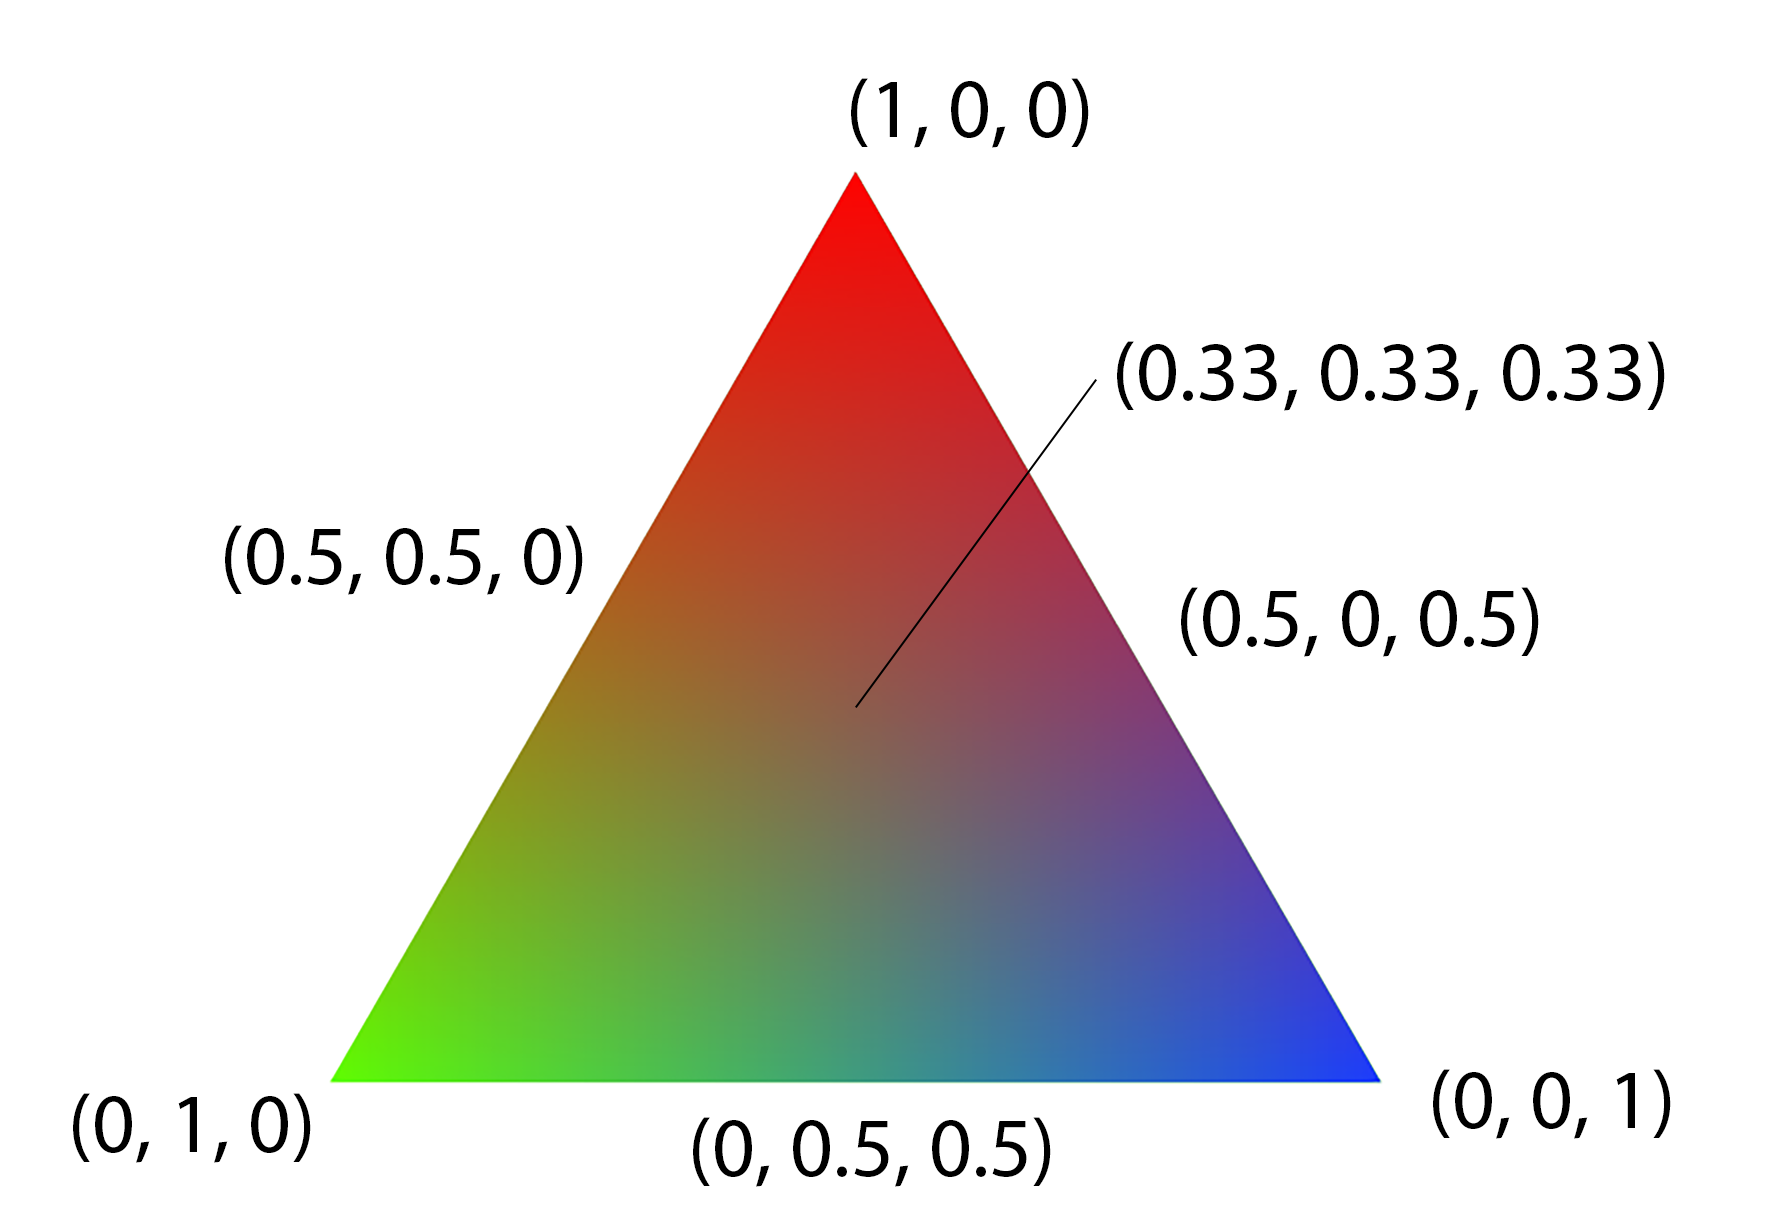
\includegraphics[width=\textwidth]{interpolation}
		\end{column}
	\end{columns}
\end{frame}


\begin{frame}{Exercise 1 - Shaders}
	\begin{itemize}
		\item Make sure you can compile and run the demos from last week
		\item Bring in the shader loading code from the following - \url{http://www.opengl-tutorial.org/beginners-tutorials/tutorial-2-the-first-triangle/}
		\item Add in a basic Vertex and Fragment shader based on the above link
		\item Compile and run the application
	\end{itemize}
\end{frame}

\begin{frame}{Exercise 2 - Working with Uniform Variables}
	\begin{itemize}
		\item Add in a Uniform variable to the fragment shader, this should be a vec4 representing the colour of the triangle
		\item Send the colour across from the Application side (C++), you can use an array of floats or GLM Library to represent the colour on the C++ side
		\item Compile and run the application
	\end{itemize}
\end{frame}

\end{document}
